% Options for packages loaded elsewhere
\PassOptionsToPackage{unicode}{hyperref}
\PassOptionsToPackage{hyphens}{url}
%
\documentclass[
]{book}
\usepackage{amsmath,amssymb}
\usepackage{lmodern}
\usepackage{ifxetex,ifluatex}
\ifnum 0\ifxetex 1\fi\ifluatex 1\fi=0 % if pdftex
  \usepackage[T1]{fontenc}
  \usepackage[utf8]{inputenc}
  \usepackage{textcomp} % provide euro and other symbols
\else % if luatex or xetex
  \usepackage{unicode-math}
  \defaultfontfeatures{Scale=MatchLowercase}
  \defaultfontfeatures[\rmfamily]{Ligatures=TeX,Scale=1}
\fi
% Use upquote if available, for straight quotes in verbatim environments
\IfFileExists{upquote.sty}{\usepackage{upquote}}{}
\IfFileExists{microtype.sty}{% use microtype if available
  \usepackage[]{microtype}
  \UseMicrotypeSet[protrusion]{basicmath} % disable protrusion for tt fonts
}{}
\makeatletter
\@ifundefined{KOMAClassName}{% if non-KOMA class
  \IfFileExists{parskip.sty}{%
    \usepackage{parskip}
  }{% else
    \setlength{\parindent}{0pt}
    \setlength{\parskip}{6pt plus 2pt minus 1pt}}
}{% if KOMA class
  \KOMAoptions{parskip=half}}
\makeatother
\usepackage{xcolor}
\IfFileExists{xurl.sty}{\usepackage{xurl}}{} % add URL line breaks if available
\IfFileExists{bookmark.sty}{\usepackage{bookmark}}{\usepackage{hyperref}}
\hypersetup{
  pdftitle={SPI-IPM Code Manual},
  pdfauthor={Chloé R. Nater},
  hidelinks,
  pdfcreator={LaTeX via pandoc}}
\urlstyle{same} % disable monospaced font for URLs
\usepackage{color}
\usepackage{fancyvrb}
\newcommand{\VerbBar}{|}
\newcommand{\VERB}{\Verb[commandchars=\\\{\}]}
\DefineVerbatimEnvironment{Highlighting}{Verbatim}{commandchars=\\\{\}}
% Add ',fontsize=\small' for more characters per line
\usepackage{framed}
\definecolor{shadecolor}{RGB}{248,248,248}
\newenvironment{Shaded}{\begin{snugshade}}{\end{snugshade}}
\newcommand{\AlertTok}[1]{\textcolor[rgb]{0.94,0.16,0.16}{#1}}
\newcommand{\AnnotationTok}[1]{\textcolor[rgb]{0.56,0.35,0.01}{\textbf{\textit{#1}}}}
\newcommand{\AttributeTok}[1]{\textcolor[rgb]{0.77,0.63,0.00}{#1}}
\newcommand{\BaseNTok}[1]{\textcolor[rgb]{0.00,0.00,0.81}{#1}}
\newcommand{\BuiltInTok}[1]{#1}
\newcommand{\CharTok}[1]{\textcolor[rgb]{0.31,0.60,0.02}{#1}}
\newcommand{\CommentTok}[1]{\textcolor[rgb]{0.56,0.35,0.01}{\textit{#1}}}
\newcommand{\CommentVarTok}[1]{\textcolor[rgb]{0.56,0.35,0.01}{\textbf{\textit{#1}}}}
\newcommand{\ConstantTok}[1]{\textcolor[rgb]{0.00,0.00,0.00}{#1}}
\newcommand{\ControlFlowTok}[1]{\textcolor[rgb]{0.13,0.29,0.53}{\textbf{#1}}}
\newcommand{\DataTypeTok}[1]{\textcolor[rgb]{0.13,0.29,0.53}{#1}}
\newcommand{\DecValTok}[1]{\textcolor[rgb]{0.00,0.00,0.81}{#1}}
\newcommand{\DocumentationTok}[1]{\textcolor[rgb]{0.56,0.35,0.01}{\textbf{\textit{#1}}}}
\newcommand{\ErrorTok}[1]{\textcolor[rgb]{0.64,0.00,0.00}{\textbf{#1}}}
\newcommand{\ExtensionTok}[1]{#1}
\newcommand{\FloatTok}[1]{\textcolor[rgb]{0.00,0.00,0.81}{#1}}
\newcommand{\FunctionTok}[1]{\textcolor[rgb]{0.00,0.00,0.00}{#1}}
\newcommand{\ImportTok}[1]{#1}
\newcommand{\InformationTok}[1]{\textcolor[rgb]{0.56,0.35,0.01}{\textbf{\textit{#1}}}}
\newcommand{\KeywordTok}[1]{\textcolor[rgb]{0.13,0.29,0.53}{\textbf{#1}}}
\newcommand{\NormalTok}[1]{#1}
\newcommand{\OperatorTok}[1]{\textcolor[rgb]{0.81,0.36,0.00}{\textbf{#1}}}
\newcommand{\OtherTok}[1]{\textcolor[rgb]{0.56,0.35,0.01}{#1}}
\newcommand{\PreprocessorTok}[1]{\textcolor[rgb]{0.56,0.35,0.01}{\textit{#1}}}
\newcommand{\RegionMarkerTok}[1]{#1}
\newcommand{\SpecialCharTok}[1]{\textcolor[rgb]{0.00,0.00,0.00}{#1}}
\newcommand{\SpecialStringTok}[1]{\textcolor[rgb]{0.31,0.60,0.02}{#1}}
\newcommand{\StringTok}[1]{\textcolor[rgb]{0.31,0.60,0.02}{#1}}
\newcommand{\VariableTok}[1]{\textcolor[rgb]{0.00,0.00,0.00}{#1}}
\newcommand{\VerbatimStringTok}[1]{\textcolor[rgb]{0.31,0.60,0.02}{#1}}
\newcommand{\WarningTok}[1]{\textcolor[rgb]{0.56,0.35,0.01}{\textbf{\textit{#1}}}}
\usepackage{longtable,booktabs,array}
\usepackage{calc} % for calculating minipage widths
% Correct order of tables after \paragraph or \subparagraph
\usepackage{etoolbox}
\makeatletter
\patchcmd\longtable{\par}{\if@noskipsec\mbox{}\fi\par}{}{}
\makeatother
% Allow footnotes in longtable head/foot
\IfFileExists{footnotehyper.sty}{\usepackage{footnotehyper}}{\usepackage{footnote}}
\makesavenoteenv{longtable}
\usepackage{graphicx}
\makeatletter
\def\maxwidth{\ifdim\Gin@nat@width>\linewidth\linewidth\else\Gin@nat@width\fi}
\def\maxheight{\ifdim\Gin@nat@height>\textheight\textheight\else\Gin@nat@height\fi}
\makeatother
% Scale images if necessary, so that they will not overflow the page
% margins by default, and it is still possible to overwrite the defaults
% using explicit options in \includegraphics[width, height, ...]{}
\setkeys{Gin}{width=\maxwidth,height=\maxheight,keepaspectratio}
% Set default figure placement to htbp
\makeatletter
\def\fps@figure{htbp}
\makeatother
\setlength{\emergencystretch}{3em} % prevent overfull lines
\providecommand{\tightlist}{%
  \setlength{\itemsep}{0pt}\setlength{\parskip}{0pt}}
\setcounter{secnumdepth}{5}
\usepackage{booktabs}
\usepackage{amsthm}
\makeatletter
\def\thm@space@setup{%
  \thm@preskip=8pt plus 2pt minus 4pt
  \thm@postskip=\thm@preskip
}
\makeatother
\ifluatex
  \usepackage{selnolig}  % disable illegal ligatures
\fi
\usepackage[]{natbib}
\bibliographystyle{apalike}

\title{SPI-IPM Code Manual}
\author{Chloé R. Nater}
\date{2021-09-30}

\begin{document}
\maketitle

{
\setcounter{tocdepth}{1}
\tableofcontents
}
\hypertarget{about-this-manual}{%
\chapter*{About this manual}\label{about-this-manual}}
\addcontentsline{toc}{chapter}{About this manual}

Briefly on the need for/value of standardized data and analyses.

Why IPMs are popular and what they are suitable for \citep{kery2011, plard2019}.

Overview over workflow, code repository \& contents of manual (Figure \ref{fig:WorkflowDiag}).

\begin{figure}

{\centering 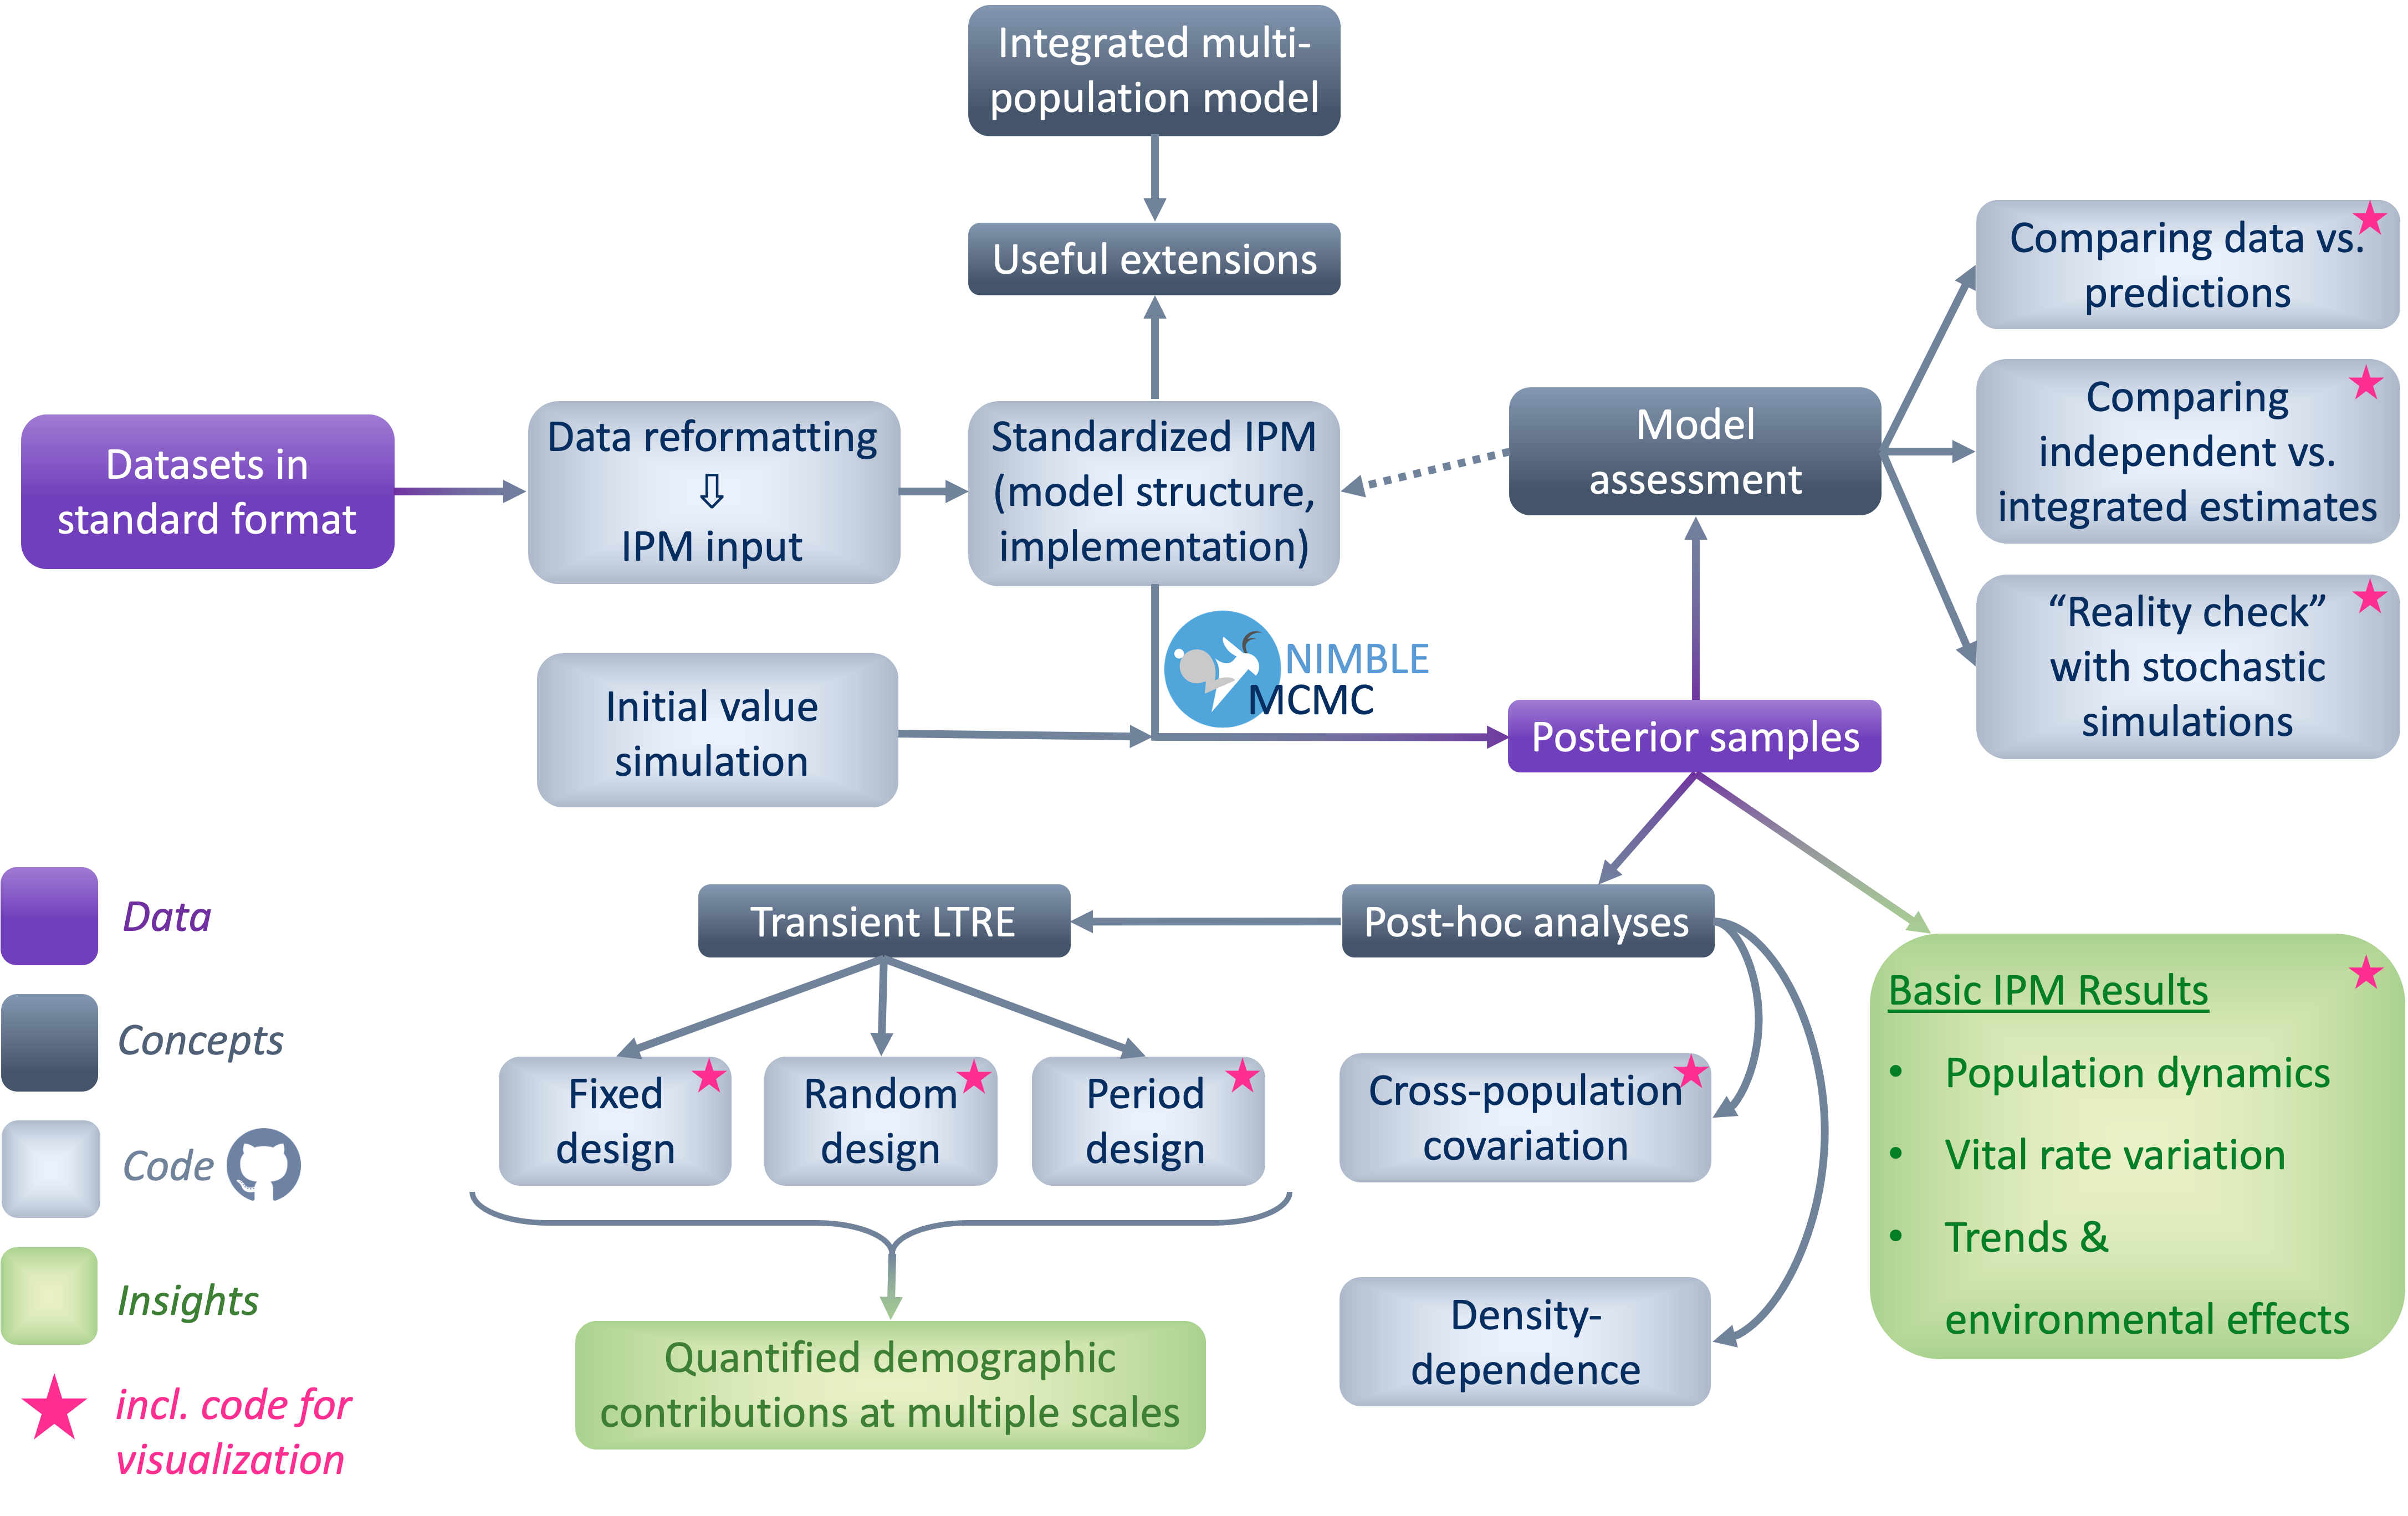
\includegraphics[width=1\linewidth]{Figures/SPI-IPM_Workflow} 

}

\caption{Schematic representation of the SPI-IPM workflow.}\label{fig:WorkflowDiag}
\end{figure}

In no way complete: great if user's analyses/adaptations become part.

How to cite.

\hypertarget{DataPrep}{%
\chapter{Preparing SPI-Birds data for Bayesian analysis}\label{DataPrep}}

Quick recap of SPI-Birds standard format and overview over data types used in IPM (+ how they relate, incl.~diagram).

\hypertarget{nest-count-data}{%
\section{Nest count data}\label{nest-count-data}}

\hypertarget{clutch-size-data}{%
\section{Clutch size data}\label{clutch-size-data}}

\hypertarget{nest-level}{%
\subsection{Nest level}\label{nest-level}}

\hypertarget{population-level}{%
\subsection{Population level}\label{population-level}}

\hypertarget{fledgling-count-data}{%
\section{Fledgling count data}\label{fledgling-count-data}}

\hypertarget{nest-level-1}{%
\subsection{Nest level}\label{nest-level-1}}

\hypertarget{population-level-1}{%
\subsection{Population level}\label{population-level-1}}

\hypertarget{mark-recapture-data}{%
\section{Mark-recapture data}\label{mark-recapture-data}}

\hypertarget{individual-capture-histories}{%
\subsection{Individual capture histories}\label{individual-capture-histories}}

\hypertarget{m-array}{%
\subsection{M-array}\label{m-array}}

\hypertarget{immigrant-count-data}{%
\section{Immigrant count data}\label{immigrant-count-data}}

\hypertarget{auxiliary-data-on-the-sampling-process}{%
\section{Auxiliary data on the sampling process}\label{auxiliary-data-on-the-sampling-process}}

\hypertarget{nest-survey-sampling-effort}{%
\subsection{Nest survey sampling effort}\label{nest-survey-sampling-effort}}

\hypertarget{capture-probability-proxies}{%
\subsection{Capture probability proxies}\label{capture-probability-proxies}}

\hypertarget{IPMCon}{%
\chapter{IPM Construction}\label{IPMCon}}

\hypertarget{open-population-model-with-2-age-classes}{%
\section{Open population model with 2 age classes}\label{open-population-model-with-2-age-classes}}

\hypertarget{model-description}{%
\subsection{Model description}\label{model-description}}

Population dynamics are represented using a female-based age-structured open
population model with a pre-breeding census in spring. At census, females are
divided into two age classes: ``yearlings'' (1-year old birds hatched during the
breeding season of the previous year) and ``adults'' (birds older than one year).
The motivation underlying this distinction is that reproductive output often
differs for these two age classes in passerine birds.
The dynamics of the female segment of the population over the time-interval from
census in year \(t\) to census in year \(t+1\) can be described with classic matrix
notation \citep{Caswell2001} as:\\

\[N_{tot,t+1} = \begin{bmatrix} N_{Y,t+1} \\ N_{A,t+1} \end{bmatrix} =
  \begin{bmatrix}
0.5F_{Y,t}sJ_t & 0.5F_{A,t}sJ_t \\
sA_t & sA_t
\end{bmatrix}\begin{bmatrix} N_{Y,t} \\ N_{A,t} \end{bmatrix} +
  \begin{bmatrix} Imm_{Y,t+1} \\ Imm_{A,t+1} \end{bmatrix}\]

\(N_{tot,t+1}\) represents the total number of yearling and adult females in the
population upon arrival in the breeding areas in year t. The total female
population size, \(N_{tot,t+1}\), is the sum of the numbers of yearling and adult
females in the population in year \(t+1\) (\(N_{Y,t+1}\) and \(N_{A,t+1}\),
respectively) and consists of local survivors and recruits from the previous
breeding season, as well as immigrant yearling (\(Imm_{Y,t+1}\)) and adult
(\(Imm_{A,t+1}\)) females.\\

\(F_{a,t}\) represents the expected number of fledglings produced by age class \(a\)
females during the breeding season in year \(t\) and is the product of several
vital rates. First, females in age class a may breed in a nestbox with
probability \(pB_{a,t}\) upon arrival to breeding areas in year \(t\). Each breeding
female may then lay a clutch containing a certain number of eggs (expected
number = \(CS_{a,t}\)), and each egg within the clutch may hatch and survive to
fledging. The probability of an egg hatching and surviving to fledging is
divided into an age-independent probability of nest success (\(pNS_t\),
probability of complete clutch failure = \(1-pNS_t\)) and a survival probability
of every egg/chick to fledging provided that the nest has not failed entirely
(\(sN_{a,t}\), with \(a\) = age of the mother). Consequently, the expected number of
fledglings produced by age class \(a\) females in year t is defined as:

\begin{equation}
F_{a,t}= pB_{a,t}\times CS_{a,t}\times pNS_{t}\times sN_{a,t}
\end{equation}\\

Fledglings that survive to the next breeding season and remain within the
population (probability = \(sJ_t\)) contribute to next year's yearling class
(\(N_{Y,t+1}\)). Yearlings and adults that survive to the next breeding season and
remain within the population (probability = \(sA_t\)) become part of next year's
adult age class (\(N_{A,t+1}\)).

\hypertarget{code-implementation-including-demographic-stochasticity}{%
\subsection{Code implementation including demographic stochasticity}\label{code-implementation-including-demographic-stochasticity}}

Population process models within IPMs are typically implemented as stochastic
models that account for randomness in the outcomes of demographic processes at
the individual level \citep[``demographic stochasticity'',][]{Caswell2001, kery2011}.
The model described here is no different, meaning that the numbers of breeders,
fledglings, and survivors are treated as binomial and Poisson random variables.

Reproduction is modelled via two sets of random variables: a binomial random
variable representing the number of breeders in age class \(a\) in year \(t\),
\(B_{a,t}\) and a Poisson random variable representing the
number of fledlings produced by breeders of age class \(a\) in year \(t\),
\(Juv_{a,t}\) . The implementation in the BUGS language used in the
SPI-IPM code (\href{https://github.com/SPI-Birds/SPI-IPM/blob/main/SPI-IPM_Code/02-04_IPM_Setup\&Run/IPMSetup.R}{\texttt{IPMSetup.R}}, lines 231-241) looks like:

\begin{Shaded}
\begin{Highlighting}[]
\ControlFlowTok{for}\NormalTok{ (t }\ControlFlowTok{in} \DecValTok{1}\SpecialCharTok{:}\NormalTok{Tmax)\{}
  \ControlFlowTok{for}\NormalTok{(a }\ControlFlowTok{in} \DecValTok{1}\SpecialCharTok{:}\NormalTok{A)\{}
    
    \DocumentationTok{\#\# 1) Breeding decision}
\NormalTok{    B[a,t] }\SpecialCharTok{\textasciitilde{}} \FunctionTok{dbin}\NormalTok{(pB[a,t], N[a,t])}
    
    \DocumentationTok{\#\# 2) Offspring production}
\NormalTok{    Juv[a,t] }\SpecialCharTok{\textasciitilde{}} \FunctionTok{dpois}\NormalTok{(B[a,t]}\SpecialCharTok{*}\NormalTok{CS[a,t]}\SpecialCharTok{*}\NormalTok{pNS[t]}\SpecialCharTok{*}\NormalTok{sN[a,t]}\SpecialCharTok{*}\FloatTok{0.5}\NormalTok{)}
\NormalTok{  \}}
\NormalTok{\}}
\end{Highlighting}
\end{Shaded}

Analogously, the numbers of local survivors -- both fledglings surviving their
first year and becoming yearlings, and yearlings and adults surviving to the
next year -- are implemented as binomial random variables (\href{https://github.com/SPI-Birds/SPI-IPM/blob/main/SPI-IPM_Code/02-04_IPM_Setup\&Run/IPMSetup.R}{\texttt{IPMSetup.R}}, lines 243-255):

\begin{Shaded}
\begin{Highlighting}[]
\ControlFlowTok{for}\NormalTok{ (t }\ControlFlowTok{in} \DecValTok{1}\SpecialCharTok{:}\NormalTok{(Tmax}\DecValTok{{-}1}\NormalTok{))\{}
  
  \DocumentationTok{\#\# 3) Annual survival of local birds}
  \CommentTok{\# Juveniles {-}\textgreater{} Yearlings}
\NormalTok{  localN[}\DecValTok{1}\NormalTok{,t}\SpecialCharTok{+}\DecValTok{1}\NormalTok{] }\SpecialCharTok{\textasciitilde{}} \FunctionTok{dbin}\NormalTok{(sJ[t], }\FunctionTok{sum}\NormalTok{(Juv[}\DecValTok{1}\SpecialCharTok{:}\NormalTok{A,t]))}
  \CommentTok{\# Yearlings/Adults {-}\textgreater{} adults}
\NormalTok{  localN[}\DecValTok{2}\NormalTok{,t}\SpecialCharTok{+}\DecValTok{1}\NormalTok{] }\SpecialCharTok{\textasciitilde{}} \FunctionTok{dbin}\NormalTok{(sA[t], }\FunctionTok{sum}\NormalTok{(N[}\DecValTok{1}\SpecialCharTok{:}\NormalTok{A,t]))}
  
  \DocumentationTok{\#\# 4) Immigration}
  \ControlFlowTok{for}\NormalTok{(a }\ControlFlowTok{in} \DecValTok{1}\SpecialCharTok{:}\NormalTok{A)\{}
\NormalTok{    N[a,t}\SpecialCharTok{+}\DecValTok{1}\NormalTok{] }\OtherTok{\textless{}{-}}\NormalTok{ localN[a,t}\SpecialCharTok{+}\DecValTok{1}\NormalTok{] }\SpecialCharTok{+}\NormalTok{ Imm[a,t}\SpecialCharTok{+}\DecValTok{1}\NormalTok{]}
\NormalTok{  \}}
\NormalTok{\}}
\end{Highlighting}
\end{Shaded}

Immigrant numbers are also treated as outcomes of stochastic processes, and
these are detailed in \protect\hyperlink{ux5cux23ux5cux23ux5cux2520Immigrantux5cux2520countux5cux2520dataux5cux2520likelihood}{2.2.5 Immigrant count data likelihood}.

\hypertarget{data-likelihoods}{%
\section{Data likelihoods}\label{data-likelihoods}}

IPMs obtain information on the population model's parameters (population sizes
and vital rates) from several different data sets. Information in each data set
is channeled into model parameters via one or multiple data likelihoods.\\
The SPI-IPM contains five data modules consisting of a total of eight data
likelihoods: nest count data (one likelihood), clutch size data (two likelihoods),
fledgling count data (three likelihoods), mark-recapture data (one likelihood),
and immigrant count data (one likelihood).
The likelihoods contained in each data module are described in detail in the
following sub-chapters. The underlying data sets are introduced in
\protect\hyperlink{DataPrep}{Chapter 1} of the manual.

\hypertarget{nest-count-data-likelihood}{%
\subsection{Nest count data likelihood}\label{nest-count-data-likelihood}}

\hypertarget{clutch-size-data-likelihoods}{%
\subsection{Clutch size data likelihoods}\label{clutch-size-data-likelihoods}}

\hypertarget{fledgling-count-data-likelihoods}{%
\subsection{Fledgling count data likelihoods}\label{fledgling-count-data-likelihoods}}

\hypertarget{mark-recapture-data-likelihood}{%
\subsection{Mark-recapture data likelihood}\label{mark-recapture-data-likelihood}}

\hypertarget{immigrant-count-data-likelihood}{%
\subsection{Immigrant count data likelihood}\label{immigrant-count-data-likelihood}}

\hypertarget{priors-and-constraints}{%
\section{Priors and constraints}\label{priors-and-constraints}}

\hypertarget{TempVar}{%
\chapter{Modelling temporal variation}\label{TempVar}}

\hypertarget{random-year-variation}{%
\section{Random year variation}\label{random-year-variation}}

\hypertarget{temporal-covariates}{%
\section{Temporal covariates}\label{temporal-covariates}}

\hypertarget{continuous-variables}{%
\subsection{Continuous variables}\label{continuous-variables}}

\hypertarget{categorical-variables}{%
\subsection{Categorical variables}\label{categorical-variables}}

\hypertarget{imputation-of-missing-covariate-values}{%
\subsection{Imputation of missing covariate values}\label{imputation-of-missing-covariate-values}}

\hypertarget{notes-on-covariate-selection}{%
\section{Notes on covariate selection}\label{notes-on-covariate-selection}}

\hypertarget{IPMImp}{%
\chapter{IPM Implementation}\label{IPMImp}}

\hypertarget{efficient-implementation-using-nimble}{%
\section{Efficient implementation using NIMBLE}\label{efficient-implementation-using-nimble}}

We use the fantastic \textbf{nimble} package \citep{devalpine2017}!

\hypertarget{simulation-of-initial-values}{%
\section{Simulation of initial values}\label{simulation-of-initial-values}}

\hypertarget{test-runs-and-full-runs-chains-iterations-burn-in-and-thinning}{%
\section{Test runs and full runs: chains, iterations, burn-in, and thinning}\label{test-runs-and-full-runs-chains-iterations-burn-in-and-thinning}}

\hypertarget{trouble-shooting-implementation-issues}{%
\section{Trouble-shooting implementation issues}\label{trouble-shooting-implementation-issues}}

\hypertarget{ModelAssm}{%
\chapter{Model Assessment}\label{ModelAssm}}

\hypertarget{assessing-chain-convergence}{%
\section{Assessing chain convergence}\label{assessing-chain-convergence}}

\hypertarget{plotting-data-vs.-predictions}{%
\section{Plotting data vs.~predictions}\label{plotting-data-vs.-predictions}}

\hypertarget{comparing-estimates-from-integrated-vs.-independent-analyses}{%
\section{Comparing estimates from integrated vs.~independent analyses}\label{comparing-estimates-from-integrated-vs.-independent-analyses}}

\hypertarget{reality-check-using-stochastic-simulations}{%
\section{``Reality check'' using stochastic simulations}\label{reality-check-using-stochastic-simulations}}

\hypertarget{other-approaches}{%
\section{Other approaches}\label{other-approaches}}

Running for additional years and comparing to non-included data, PPCs, etc.

\hypertarget{ResultsViz}{%
\chapter{Visualizing and interpreting direct IPM outputs}\label{ResultsViz}}

\hypertarget{population-trajectories}{%
\section{Population trajectories}\label{population-trajectories}}

\hypertarget{within-population-variation-in-vital-rates}{%
\section{Within-population variation in vital rates}\label{within-population-variation-in-vital-rates}}

\hypertarget{age-class-specific-averages}{%
\subsection{Age-class-specific averages}\label{age-class-specific-averages}}

\hypertarget{year-by-year-variation}{%
\subsection{Year-by-year variation}\label{year-by-year-variation}}

\hypertarget{between-population-variation-in-vital-rates}{%
\section{Between-population variation in vital rates}\label{between-population-variation-in-vital-rates}}

\hypertarget{population-specific-averages}{%
\subsection{Population-specific averages}\label{population-specific-averages}}

\hypertarget{year-by-year-variation-1}{%
\subsection{Year-by-year variation}\label{year-by-year-variation-1}}

\hypertarget{covariate-effects}{%
\section{Covariate effects}\label{covariate-effects}}

\hypertarget{AddAnalyses}{%
\chapter{Follow-up Analyses}\label{AddAnalyses}}

\hypertarget{testing-for-time-trends}{%
\section{Testing for time-trends}\label{testing-for-time-trends}}

\hypertarget{testing-for-density-dependence}{%
\section{Testing for density-dependence}\label{testing-for-density-dependence}}

\hypertarget{investigating-cross-population-covariation}{%
\section{Investigating cross-population covariation}\label{investigating-cross-population-covariation}}

\hypertarget{quantifying-demographic-contributions-to-short-term-population-dynamics}{%
\section{Quantifying demographic contributions to short term population dynamics}\label{quantifying-demographic-contributions-to-short-term-population-dynamics}}

\hypertarget{year-by-year-variation-in-population-growth-rate-random-design-ltre}{%
\subsection{Year-by-year variation in population growth rate (random design LTRE)}\label{year-by-year-variation-in-population-growth-rate-random-design-ltre}}

\hypertarget{year-to-year-differences-in-population-growth-rate-fixed-design-ltre}{%
\subsection{Year-to-year differences in population growth rate (fixed design LTRE)}\label{year-to-year-differences-in-population-growth-rate-fixed-design-ltre}}

\hypertarget{quantifying-demographic-contributions-to-long-term-population-trends}{%
\section{Quantifying demographic contributions to long-term population trends}\label{quantifying-demographic-contributions-to-long-term-population-trends}}

\hypertarget{differences-in-population-trajectories-between-time-periods-period-design-ltre}{%
\subsection{Differences in population trajectories between time periods (period design LTRE)}\label{differences-in-population-trajectories-between-time-periods-period-design-ltre}}

\hypertarget{differences-in-population-trajectories-between-locations-period-design-ltre-with-time-by-space-substitution}{%
\subsection{Differences in population trajectories between locations (period design LTRE with time-by-space substitution)}\label{differences-in-population-trajectories-between-locations-period-design-ltre-with-time-by-space-substitution}}

\hypertarget{ExtOutlook}{%
\chapter{Useful extensions and outlook}\label{ExtOutlook}}

\hypertarget{adapting-the-population-model-for-your-speciespopulation}{%
\section{Adapting the population model for your species/population}\label{adapting-the-population-model-for-your-speciespopulation}}

\hypertarget{accounting-for-multiple-broods-per-bird-per-year}{%
\subsection{Accounting for multiple broods per bird per year}\label{accounting-for-multiple-broods-per-bird-per-year}}

\hypertarget{altering-age-structure}{%
\subsection{Altering age structure}\label{altering-age-structure}}

\hypertarget{individual-heterogeneity-beyond-age-sex-traits-and-more}{%
\subsection{Individual heterogeneity beyond age: sex, traits, and more}\label{individual-heterogeneity-beyond-age-sex-traits-and-more}}

\hypertarget{including-additional-data-and-informative-priors}{%
\section{Including additional data and informative priors}\label{including-additional-data-and-informative-priors}}

\hypertarget{including-partially-observed-age-information}{%
\subsection{Including partially observed age information}\label{including-partially-observed-age-information}}

\hypertarget{making-the-most-of-auxiliary-knowledge-about-immigrantsdispersers}{%
\subsection{Making the most of auxiliary knowledge about immigrants/dispersers}\label{making-the-most-of-auxiliary-knowledge-about-immigrantsdispersers}}

\hypertarget{letting-published-values-help-with-estimation-when-data-is-sparse}{%
\subsection{Letting published values help with estimation when data is sparse}\label{letting-published-values-help-with-estimation-when-data-is-sparse}}

\hypertarget{building-on-the-multi-population-perspective}{%
\section{Building on the multi-population perspective}\label{building-on-the-multi-population-perspective}}

\hypertarget{joint-analysis-of-data-from-several-populations}{%
\subsection{Joint analysis of data from several populations}\label{joint-analysis-of-data-from-several-populations}}

\hypertarget{modelling-cross-population-covariation}{%
\subsection{Modelling cross-population covariation}\label{modelling-cross-population-covariation}}

\hypertarget{estimating-hyper-parameters-in-large-scale-analyses}{%
\subsection{Estimating hyper-parameters in large-scale analyses}\label{estimating-hyper-parameters-in-large-scale-analyses}}

\hypertarget{unlocking-the-secrets-of-dispersal}{%
\subsection{Unlocking the secrets of dispersal}\label{unlocking-the-secrets-of-dispersal}}

  \bibliography{book.bib,packages.bib}

\end{document}
